\documentclass[a4paper]{article}
\usepackage[utf8]{inputenc}
\usepackage{amsmath}
\usepackage{polski}
\usepackage[polish]{babel}
\usepackage[T1]{fontenc}
\usepackage[a4paper,top=3cm,bottom=2cm,left=3cm,right=3cm,marginparwidth=1.75cm]{geometry}
\usepackage{graphicx}
\usepackage{float}
\usepackage{longtable}
\usepackage{pdflscape}
\usepackage[backend=bibtex]{biblatex}
\graphicspath{{../img/}}

\title{Optymalizacja fabryki z wykorzystaniem algorytmu immunologicznego (selekcji klonalnej)}
\author{Artur Bauer \and Kamil Szostek \and Sławomir Goździewski \and Wiktor Filipiak}
\date{\today}

\usepackage[pdftex,
            pdfauthor={Artur Bauer \& Kamil Szostek \& Sławomir Goździewski \& Wiktor Filipiak},
            pdftitle={\@title},
            pdfsubject={Glebokie uczenie i inteligencja obliczeniowa},
            pdfkeywords={Automatyka i Robotyka},
            pdfproducer={Latex},
            pdfcreator={pdflatex}]{hyperref}

\bibliography{citations.bib}

\begin{document}
%--------------------------------------------------------%
%	COVER PAGE
%--------------------------------------------------------%

\begin{titlepage}
\makeatletter

  \newcommand{\HRule}{\rule{\linewidth}{0.5mm}} % Defines a new command for the horizontal lines, change thickness here

  \center % Center everything on the page


%	HEADING SECTION

  \textsc{\LARGE Akademia Górniczo-Hutnicza}\\[1.5cm] % Name of your university/college
  \textsc{\Large  Głębokie uczenie i inteligencja obliczeniowa }\\[0.5cm] % Major heading such as course name
  \textsc{\large Automatyka i Robotyka II Stopień}\\[0.5cm] % Minor heading such as course title
  \textsc{2019/2020}\\[0.5cm] % Minor heading such as course title

%	TITLE SECTION

  \vspace{1.5 cm}
  \HRule \\[0.4cm]
  { \huge \bfseries \@title} \\[0.4cm] % Title of your document
  \HRule \\[1.5cm]
 
%	AUTHOR SECTION

  {\em\Large\textbf Skład zespołu:}\\
  \vspace{.5 cm}
    Artur Bauer\\
    Kamil Szostek\\
    Sławomir Goździewski\\
    Wiktor Filipiak
  \vspace{1.5 cm}
  
  
  {\em\Large\textbf Opiekun:}\\
  \vspace{.5 cm}
  dr hab. inż. Joanna Kwiecień
  
%	DATE SECTION

  \vspace{1.5 cm}
  {\large Złożono: \@date}\\[3cm] % Date, change the \today to a set date if you want to be precise


\vfill % Fill the rest of the page with whitespace

\end{titlepage}

%-----------------------------------------------------------------

\newpage

\tableofcontents

\newpage
\section{Wstęp}
\subsection{Model fabryki}\label{factory}

\begin{figure}[ht]
\centering
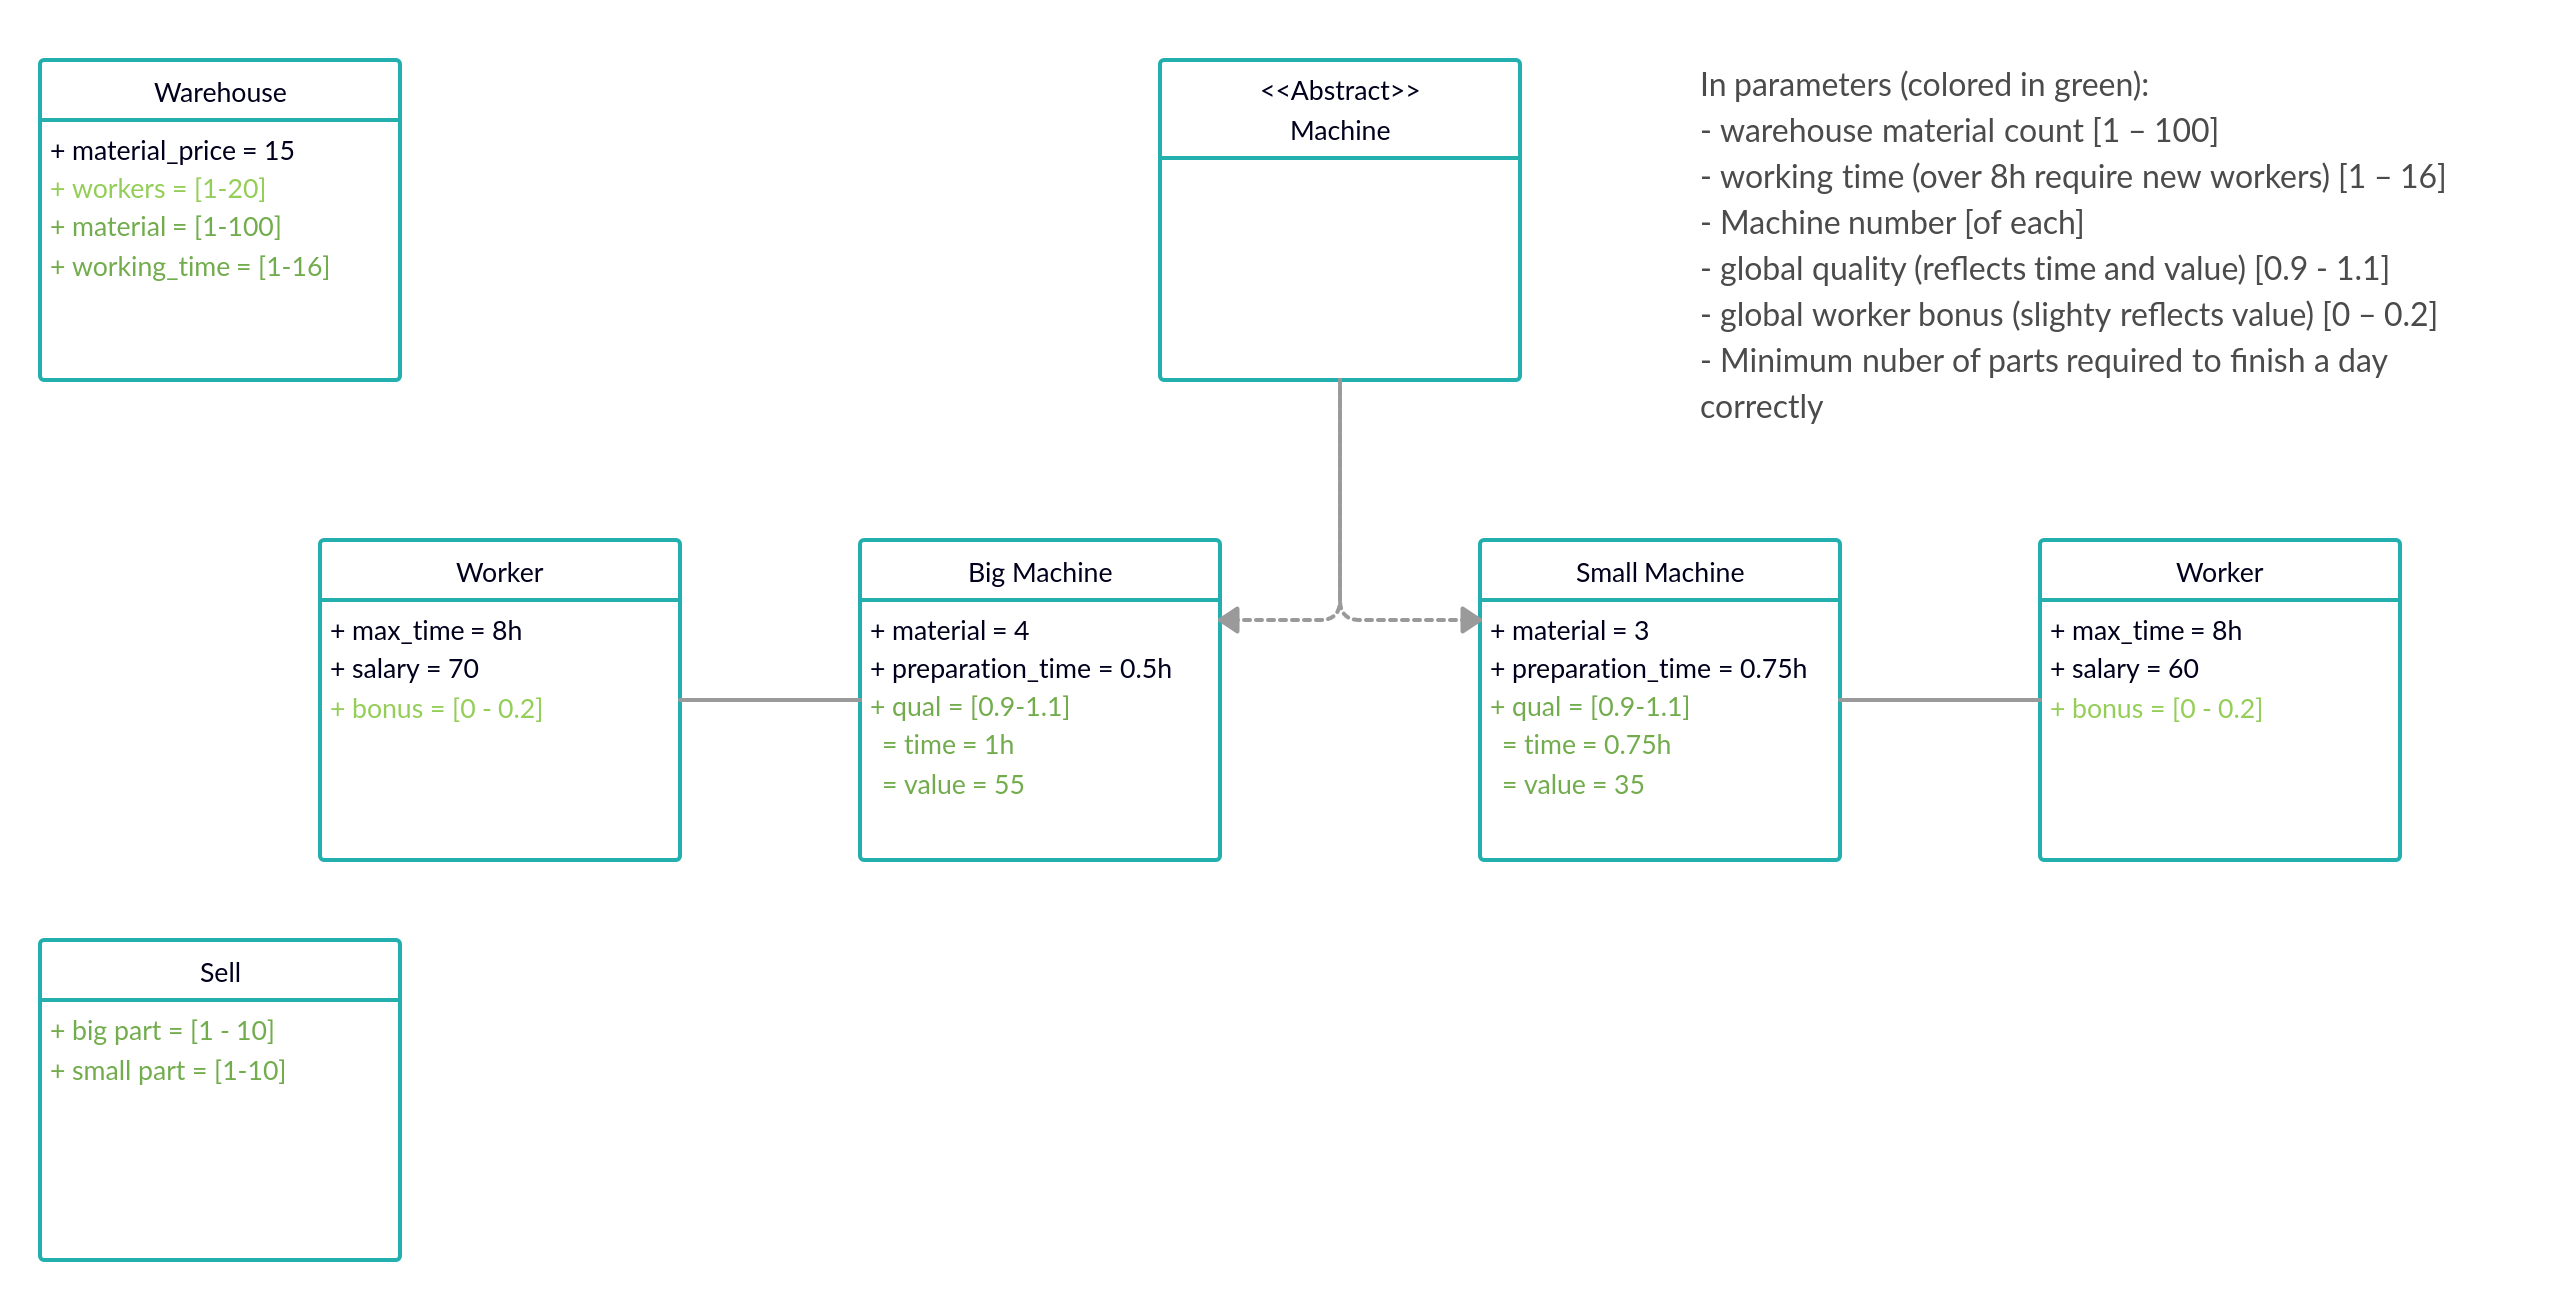
\includegraphics[width=.7\textwidth]{Factory_scheme.png}
\caption{Schemat fabryki}
\end{figure}

\subsubsection{Funkcja celu fabryki:}\label{factory-main-goal-function}

$$Income = \sum^{n_p}_{i=1}(p_i*(v_i-m_i*m_p)) - (1+b_i)*\sum^{n_w}_{i = 1}(w_i*s_i *t_{wi}) - m_r*m_p - punish$$

Gdzie:
\begin{itemize}
    \item $n_p$ -- ilość rodzajów części
    \item $p_i (n_m)$ -- ilość wyprodukowanych części i-tego typu
    \item $v_i(v_{bi}, t_{wi},t_{bi},w_q)$ -- wartość części i-tego typu
    \item $m_i$ -- liczba surowca potrzebna do wytworzenia elementu i-tego typu
    \item $m_p$ -- cena surowca
    \item $n_w$ -- liczba rodzajów pracowników
    \item $w_i$ -- liczba pracowników i-tego rodzaju
    \item $s_i$ -- wypłata pracownika i-tego rodzaju
    \item $b$ -- premia pracownicza
    \item $m_r(p_i,n_m)$ -- pozostały materiał
    \item $p_{i_{min}}$ -- minimalna ilość elementów do wytworzenia i uniknięcia kary
    \item $p_{i_{max}}$ -- maksymalna ilość wytworzonych elementów
    \item $n_m$ -- liczba surowca na początek dnia
\end{itemize}
\subsubsection{Kara}
$punish = p_{un}*\sum^{n_p}_{i=1}(p_{num_i})*v_i$

$p_{num_i}= \left\{\begin{matrix} 0  \;\quad\quad\quad\quad  \textrm{if} \quad  p_{i_{min}}-p_i \leq  0    \\ p_{i_{min}}-p_i  \quad  \textrm{if} \quad  p_{i_{min}}-p_i >  0  \end{matrix}\right.$

Gdzie: 
\begin{itemize}
    \item $p_{un}$ -- współczynnik kary
    \item $p_{num_i}(p_{i_{min}}, p_i)$ -- liczba elementów i-tego typu dla których naliczana jest kara
\end{itemize}
\subsubsection{Liczba pracowników}

Liczba pracowników i-tego typu jest równa ilości maszyn i-tego typu:

$n_p = n_w$

\subsubsection{Maksymalna ilość elementów}\label{max-number-of-items}

Niezbędna ilość elementów i-tego typu:

$\sum^{n_p}_{i=1} p_{i_{max}} * m_i< n_m$

\subsubsection{Rzeczywisty czas pracy maszyny na 1 produkt}\label{real-working-time-of-the-i-type-machineemployee-for-one-product} 
$t_{wi} = t_{pi} + p_i * t_{bi}$

\subsection{Parametry modelu}\label{model-assumption}

\begin{longtable}[c]{lll}
Parametr & oznaczenie & wartość\\ \hline
Ilość surowców & $n_m$ & [$x$ - 100]\\
Koszt surowca & $m_p$ & 15\\
Czas pracy & $t_f$ & [1 - 16]\\
Minimalna ilość dużych części & $p_{0_{min}}$ & [0 - 10]\\
Minimalna ilość małych części & $p_{1_{min}}$ & [0 -10]\\
Wypłata operatora dużej maszyny & $s_0$ & 70\\
Wymagana ilość materiału na duży element & $m_0$ & 4\\
Czas przygotowania dużej maszyny & $t_{p0}$ & 30 min\\
Wartość dużego elementu & $v_{b0}$ & 50\\
Podstawowy czas pracy na duży element & $t_{b0}$ & 1h\\
Liczba dużych maszyn & $c_0$ & [0 - 10]\\
Wypłata operatora małej maszyny & $s_1$ & 60\\
Ilość surowca na mały element & $m_1$ & 3\\
Czas przygotowania małej maszyny & $t_{p1}$ & 45 min\\
Wartość małego elementu & $v_{b1}$ & 35\\
Czas wytworzenia małego elementu & $t_{b1}$ & 45 min\\
Ilość małych maszyn & $c_1$ & [0 - 10]\\
Maksymalny czas pracy pracownika & $t_w$ & 8h\\
Bonus pracowniczy & b & [0.0 - 0.2]\\
Współczynnik kary & $p_{un}$ & 1.5
\end{longtable}

Gdzie:
\begin{itemize}
    \item $x$ -- ilość wymaganych elementów * koszt części 
    \item Parametry wejściowe podane są w kwadratowych nawiasach
    \item Pracownik jest zatrudniony na pełen etat (8h płacone z góry)
    \item Pierwsza i druga zmiana są identyczne w ilość i rodzaj maszyn i pracowników
    \item Rezerwujemy surowce na wymagane elementy
    \item Wszystkie elementy ponad wymaganą liczbę są czystym dochodem
\end{itemize}


\section{Badany problem}
\subsection{Przegląd literatury}
Artykuł dotyczy algorytmu selekcji klonalnej stosowanej do optymalizacji w elektromagnetyce. Autorzy prezentują ich własną koncepcję kodowanego algorytmu selekcji klonalnej, który może zostać użyty w elektromagnetycznej optymalizacji projektu, a także sposób działania algorytmu dla problemu "The TEAM Workshop problem 22”.\cite{1430953}.


Artykuł przedstawia użycie algorytmów sztucznych systemów immunologicznych w przemyśle. Porównuje on algorytmy sztucznej inteligencji z algorytmem klonowania do algorytmu z mechanizmem uczenia społecznego. Zmieniając wzmocnienie, czas zdwojenia oraz czas wyprzedzenia dobierają one nastawy regulatora PID \cite{wang_artificial_2017}.


Artykuł przedstawia zastosowanie sztucznego systemu immunologicznego w aplikacji przemysłowej. Na postawie parametrów obróbki (siła, moment, itp.) oraz zakłócenia (wibracje, itp.) autorzy wykrywają uszkodzenie narzędzia. Wykorzystywany jest algorytm sztucznego systemu immunologicznego wykorzystuje do działania algorytm selekcji negatywnej \cite{dasgupta1999artificial}.


Artykuł przedstawia użycie algorytmów sztucznych systemów immunologicznych w przemyśle. Porównuje on algorytmy sztucznej inteligencji z algorytmem klonowania do algorytmu z mechanizmem uczenia społecznego. Zmieniając wzmocnienie, czas zdwojenia oraz czas wyprzedzenia dobierają one nastawy regulatora PID \cite{wang_artificial_2017}.


Artykuł przedstawia działanie sztucznego systemu immunologicznego (AIS) w przypadku rozwiązania pojemnościowego problemu marszrutyzacji. Celem było znalezienie odpowiedniego zestawienia parametrów algorytmu selekcji klonalnej w celu rozwiązania problemu poprzez podejście eksperymentalne. W artykule oprócz działania AIS, opisano także działanie innych metod rozwiązujących dwadzieścia instancji problemu i przedstawiono wyniki pod względem jakości rozwiązań oraz wykorzystanego czasu obliczeniowego \cite{thapatsuwan}.


Artykuł przedstawia użycie Algorytmu Selekcji Klonalnej w zastosowaniach inżynierskich. Opisane w nim jest działanie algorytmu od strony teoretycznej, a także działanie zaimplementowanego przez autorów algorytmu przy rozwiązywaniu trzech różnych problemów: binarnego rozpoznawania znaków, wielomodalnej optymalizacji funkcji -
$f(x, y) = x.\sin{4 \pi x} - y.\sin{4 \pi y + \pi} + 1$
i problemu komiwojażera dla 30 miast \cite{de_castro}.


Artykuł przedstawia użycie Algorytmu Selekcji Klonalnej do optymalizacji ułożenia terenu budowy. Zaprezentowany algorytm minimalizuje koszty produkcji i dystans przebyty pomiędzy n obiektami zaprezentowanymi za pomocą macierzy permutacji o wymiarach n x n \cite{WANG2016267}.


Artykuł dotyczy zastosowania algorytmu selekcji klonalnej w celu określenia optymalnych punktów pracy w niskonapięciowych, hybrydowych mikrosieciach AC/DC. Celem było zminimalizowanie strat mocy czynnej, kosztów eksploatacji oraz optymalizacja napięcia węzłowego \cite{rokicki}.


\section{Diagram UML fabryki}
\begin{figure}[ht]
\centering
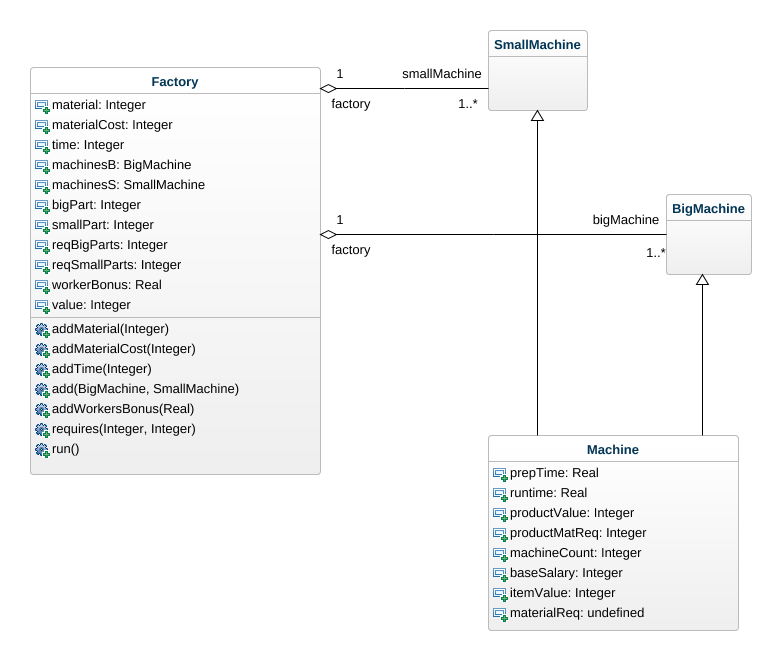
\includegraphics[width=.7\textwidth]{UML_Model.png}
\caption{Diagram UML}
\end{figure}


\newpage
\printbibliography

\end{document}
